% This must be in the first 5 lines to tell arXiv to use pdfLaTeX, which is strongly recommended.
\pdfoutput=1
% In particular, the hyperref package requires pdfLaTeX in order to break URLs across lines.

\documentclass[11pt]{article}

% Change "review" to "final" to generate the final (sometimes called camera-ready) version.
% Change to "preprint" to generate a non-anonymous version with page numbers.
\usepackage[review]{acl}

% Standard package includes
\usepackage{times}
\usepackage{latexsym}
\usepackage{float} % Added for [H] placement option

% For proper rendering and hyphenation of words containing Latin characters (including in bib files)
\usepackage[T1]{fontenc}
% For Vietnamese characters
% \usepackage[T5]{fontenc}
% See https://www.latex-project.org/help/documentation/encguide.pdf for other character sets

% This assumes your files are encoded as UTF8
\usepackage[utf8]{inputenc}

% This is not strictly necessary, and may be commented out,
% but it will improve the layout of the manuscript,
% and will typically save some space.
\usepackage{microtype}

% This is also not strictly necessary, and may be commented out.
% However, it will improve the aesthetics of text in
% the typewriter font.
\usepackage{inconsolata}

%Including images in your LaTeX document requires adding
%additional package(s)
\usepackage{graphicx}
\usepackage{booktabs} % For professional quality tables
\usepackage{amsmath}  % For math commands like \text
\usepackage{longtable} % For tables that span multiple pages
\usepackage{caption} % For captions, especially in longtable

% If the title and author information does not fit in the area allocated, uncomment the following
%
%\setlength\titlebox{<dim>}
%
% and set <dim> to something 5cm or larger.

\title{Synthetic Student Responses: LLM-Extracted Features for IRT Difficulty Parameter Estimation}

% Author information can be set in various styles:
% For several authors from the same institution:
% \author{Author 1 \and ... \and Author n \\
%         Address line \\ ... \\ Address line}
% if the names do not fit well on one line use
%         Author 1 \\ {\bf Author 2} \\ ... \\ {\bf Author n} \\
% For authors from different institutions:
% \author{Author 1 \\ Address line \\  ... \\ Address line
%         \And  ... \And
%         Author n \\ Address line \\ ... \\ Address line}
% To start a separate ``row'' of authors use \AND, as in
% \author{Author 1 \\ Address line \\  ... \\ Address line
%         \AND
%         Author 2 \\ Address line \\ ... \\ Address line \And
%         Author 3 \\ Address line \\ ... \\ Address line}

\author{Matías Hoyl \
  School of Education, Stanford University \
  % Affiliation / Address line 2 \
  % Affiliation / Address line 3 \
  \texttt{mhoyl@stanford.edu}}

%\author{
%  \textbf{First Author\textsuperscript{1}},
%  \textbf{Second Author\textsuperscript{1,2}},
%  \textbf{Third T. Author\textsuperscript{1}},
%  \textbf{Fourth Author\textsuperscript{1}},
%\\
%  \textbf{Fifth Author\textsuperscript{1,2}},
%  \textbf{Sixth Author\textsuperscript{1}},
%  \textbf{Seventh Author\textsuperscript{1}},
%  \textbf{Eighth Author \textsuperscript{1,2,3,4}},
%\\
%  \textbf{Ninth Author\textsuperscript{1}},
%  \textbf{Tenth Author\textsuperscript{1}},
%  \textbf{Eleventh E. Author\textsuperscript{1,2,3,4,5}},
%  \textbf{Twelfth Author\textsuperscript{1}},
%\\
%  \textbf{Thirteenth Author\textsuperscript{3}},
%  \textbf{Fourteenth F. Author\textsuperscript{2,4}},
%  \textbf{Fifteenth Author\textsuperscript{1}},
%  \textbf{Sixteenth Author\textsuperscript{1}},
%\\
%  \textbf{Seventeenth S. Author\textsuperscript{4,5}},
%  \textbf{Eighteenth Author\textsuperscript{3,4}},
%  \textbf{Nineteenth N. Author\textsuperscript{2,5}},
%  \textbf{Twentieth Author\textsuperscript{1}}
%\\
%\\
%  \textsuperscript{1}Affiliation 1,
%  \textsuperscript{2}Affiliation 2,
%  \textsuperscript{3}Affiliation 3,
%  \textsuperscript{4}Affiliation 4,
%  \textsuperscript{5}Affiliation 5
%\\
%  \small{
%    \textbf{Correspondence:} \href{mailto:email@domain}{email@domain}
%  }
%}

\begin{document}
\maketitle
\begin{abstract}
Educational assessment relies heavily on knowing question difficulty, traditionally determined through resource-intensive pre-testing with students. This creates significant barriers for both classroom teachers and assessment developers. We investigate whether Item Response Theory difficulty parameters can be accurately estimated without student testing by modeling the response process and explore the relative contribution of different feature types to prediction accuracy. Our approach combines traditional linguistic features with pedagogical insights extracted using Large Language Models (LLMs), including solution step count, required mathematical skills, cognitive complexity, and potential misconceptions. We implement a two-stage process: first training a neural network to predict how students would respond to questions, then deriving difficulty parameters from these simulated response patterns. Using a dataset of over 250,000 student responses to mathematics questions, our model achieves a Pearson correlation of 0.85 between predicted and actual difficulty parameters on completely unseen questions. 
\end{abstract}

\section{Introduction}

Educational assessment plays a vital role in teaching and learning, but creating high-quality questions requires knowing their difficulty level—how challenging they are for students with different abilities. Currently, determining question difficulty requires extensive pre-testing with students followed by statistical analysis, an approach that is effective but creates significant delays and costs in developing new assessments.

For teachers developing classroom assessments, this process is often impractical, leading to tests with unknown psychometric properties. For large-scale assessment programs, the pre-testing requirement consumes substantial resources and limits the speed at which new content can be developed. Both scenarios highlight the need for methods that can predict question difficulty without requiring actual student testing.

This study addresses two specific research questions:
\begin{itemize}
    \item How effectively can we estimate Item Response Theory difficulty parameters without student testing by modeling the student response process?
    \item To what extent do different feature types (LLM-extracted pedagogical features, linguistic characteristics, and semantic embeddings) contribute to the accuracy of difficulty predictions?
\end{itemize}

Rather than treating difficulty prediction as a direct regression problem, which is what most existing research does, we take an approach that mirrors how difficulty emerges in practice—through patterns of student responses.

Our method combines conventional question features with pedagogical insights extracted using Large Language Models (LLMs). These AI tools analyze questions to identify solution steps, required mathematical skills, cognitive complexity, and potential student misconceptions—aspects typically assessed by human experts. By embedding this pedagogical knowledge in our predictions, we create a system that better reflects how questions function in educational settings.

The remainder of this paper is organized as follows. Section 2 reviews related work on difficulty prediction, highlighting existing approaches and gaps in the literature. Section 3 describes our dataset, which contains over 250,000 student responses to mathematics questions. Section 4 outlines our methodology, including feature engineering and our neural network architecture. Section 5 presents our experimental results, demonstrating the effectiveness of our approach. Finally, Section 6 discusses the implications of our findings, acknowledges limitations, and suggests directions for future research.

\section{Related Work}

\subsection{Text-based Features for Difficulty Prediction}

Traditional difficulty estimation approaches rely on either expert judgment, which has proven inconsistent and subjective \citep{rudner2010implementing, impara1998teachers}, or statistical calibration through student pre-testing using Item Response Theory (IRT) models \citep{rasch1960}. While the latter provides more reliable estimates, it introduces significant delays and resource demands, creating development bottlenecks. These limitations have motivated research into automated approaches that predict item difficulty directly from question text, potentially eliminating the need for extensive pre-testing.

\subsubsection{Linguistic Features}

Linguistic characteristics of questions are strongly associated with their difficulty. Some studies have extracted lexical, syntactic, and semantic features to predict question complexity \citep{alkhuzaey2023text, choi2020predicting}. Common linguistic features include:

\begin{itemize}
    \item \textbf{Lexical features:} Word count, word frequency, word length, and vocabulary difficulty \citep{yaneva2019predicting, benedetto2020framework}
    \item \textbf{Syntactic features:} Sentence length, syntactic complexity, and grammatical structures \citep{choi2020predicting}
    \item \textbf{Semantic features:} Concept density, abstraction level, and semantic similarity between options \citep{bulut2023evaluating}
\end{itemize}

\subsubsection{Domain-specific Features}

Features specific to certain domains have been shown to improve prediction accuracy:

\begin{itemize}
    \item \textbf{Mathematics:} Number of mathematical symbols, presence of graphs or figures, computation complexity \citep{benedetto2020r2de}
    \item \textbf{Reading comprehension:} Text layout, presence of contextual cues, relationship between passages and questions \citep{lawrence2022reading}
    \item \textbf{Multiple-choice questions:} Similarity between options, plausibility of distractors \citep{kurdi2016experimental, yaneva2018automatic}
\end{itemize}

\subsection{Machine Learning Approaches for Difficulty Prediction}

Early approaches to difficulty prediction relied on deterministic methods or simple regression models. Recent advances have introduced increasingly sophisticated machine learning techniques.

\subsubsection{Classical Machine Learning Methods}

Traditional machine learning algorithms have been widely applied to the challenge of difficulty prediction. Linear and logistic regression models have proven effective in establishing relationships between text features and difficulty levels, as demonstrated by \citet{yaneva2019predicting} in their work on high-stakes medical exams. More sophisticated approaches include the R2DE model proposed by \citet{benedetto2020r2de}, which leverages random forests to simultaneously predict both IRT difficulty and discrimination parameters based on TF-IDF features extracted from question text. The literature also shows that feature-based ensemble methods have achieved notable success across various educational domains, with \citet{yaneva2019predicting} demonstrating that combining different feature types can enhance prediction accuracy compared to single-feature approaches.

\subsubsection{Neural Network Models}

Deep learning approaches have shown promise for difficulty prediction in recent years. Recurrent Neural Networks with LSTM architectures effectively capture sequential patterns in question text \citep{huang2017question}, while the Document-enhanced Attention Network (DAN) improves accuracy by enriching questions with relevant domain documents \citep{qiu2019question}. Additionally, \citet{xue2020predicting} demonstrated that models pre-trained on related tasks like response time prediction can be successfully fine-tuned for difficulty estimation, transferring knowledge between educational assessment tasks.

\subsubsection{Transformer-based Approaches}

The most recent research has explored transformer-based models for difficulty prediction, leveraging their superior ability to capture contextual relationships. \citet{benedetto2021transformers} compared BERT and DistilBERT models for difficulty estimation, finding that transformer models outperform previous approaches by up to 6.5\% in terms of RMSE. Building on this work, \citet{gombert2024predicting} employed scalar-mixed transformer encoders with specialized regression heads, showing significant improvements over baseline models. Further advancing the field, \citet{kapoor2025prediction} incorporated embeddings from various LLMs (ModernBERT, BERT, and LLAMA) alongside linguistic features, achieving a correlation of 0.77 between true and predicted difficulty.

A key advantage of transformer models is their ability to capture complex semantic relationships within text without requiring extensive feature engineering. \citet{aradelli2020transformers} demonstrated that fine-tuning pre-trained transformers on domain-specific corpora further enhances prediction accuracy. These approaches represent the current state-of-the-art in difficulty prediction, combining the contextual understanding capabilities of transformer architectures with specialized training techniques to achieve unprecedented levels of accuracy in estimating question difficulty from text alone.

\subsection{Feature Extraction Using Language Models}

Recent studies have explored the use of Large Language Models (LLMs) not just for prediction but also for feature extraction:

\begin{itemize}
    \item \textbf{Procedural complexity:} Using LLMs to quantify the number of steps required to solve problems \citep{liu2023improving} % Using citep as textcite was used without parenthesis in source
    \item \textbf{Skill identification:} Extracting the specific skills required to answer questions \citep{didolkar2024metacognitive} % Using citep as textcite was used without parenthesis in source
    \item \textbf{Cognitive level assessment:} Classifying questions according to Bloom's taxonomy \citep{scaria2024automated} % Using citep as textcite was used without parenthesis in source
    \item \textbf{Misconception analysis:} Identifying potential student misconceptions associated with questions \citep{sadihin2024proposalml} % Using citep as textcite was used without parenthesis in source
\end{itemize}

These approaches leverage the reasoning capabilities of LLMs to extract pedagogically meaningful features that might be difficult to capture through conventional feature engineering.

\subsection{Gaps in Current Research}

Despite significant advances in difficulty prediction methods, two important gaps remain in current research.

First, transformer-based models have shown remarkable results, but there has been limited exploration of using Large Language Models (LLMs) to extract pedagogically meaningful features from questions. Most studies rely on conventional linguistic features or embedding-based approaches, neglecting LLMs' potential to identify complex attributes like procedural complexity, specific skills, cognitive levels, and potential misconceptions.

LLM-extracted features could provide richer signals about question characteristics that traditional feature engineering struggles to capture. While a few studies exploring this approach show promise, it remains underutilized in difficulty prediction literature.

Second, most research approaches difficulty prediction as a direct regression problem, predicting difficulty parameters directly from question text and features. This bypasses a crucial intermediate step: modeling how students with varying abilities would actually respond to these questions.

Few studies have explored first simulating student responses and then deriving difficulty parameters from these simulated patterns. This simulation-based approach better mimics how question difficulty emerges in educational settings and provides a more interpretable model that captures both question characteristics and student abilities, while also producing additional metrics beyond difficulty.

This gap presents an opportunity for more robust difficulty estimation methods. A model that successfully simulates student responses could estimate difficulty parameters for unseen questions without requiring actual student testing, reducing resource burdens while maintaining psychometric validity.

Our study addresses both gaps by (1) using LLMs to extract complex pedagogical features and (2) developing a neural network that first predicts student responses before deriving IRT difficulty parameters from these predictions.

\section{Data}

The dataset used in this study originates from Zapien, an adaptive educational technology platform based in Chile, focused on helping students learn mathematics. The dataset contains 280,979 answers from approximately 2,000 students across 50+ schools. Each record represents an interaction between a student and the platform, providing information on the student's skill level, question attributes, and outcomes.

Key features of the dataset include student demographic information and skill levels, question characteristics (options, text) and difficulty metrics, response data including correctness and timing, topic and subject categorization, and school and grade-level information.

\section{Methods}

We developed a pipeline that combines traditional machine learning techniques with features extracted using large language models (LLMs). Our approach integrates student-specific information, question characteristics, and interaction patterns to create a robust predictive framework.

\begin{figure}[H]
    \centering
    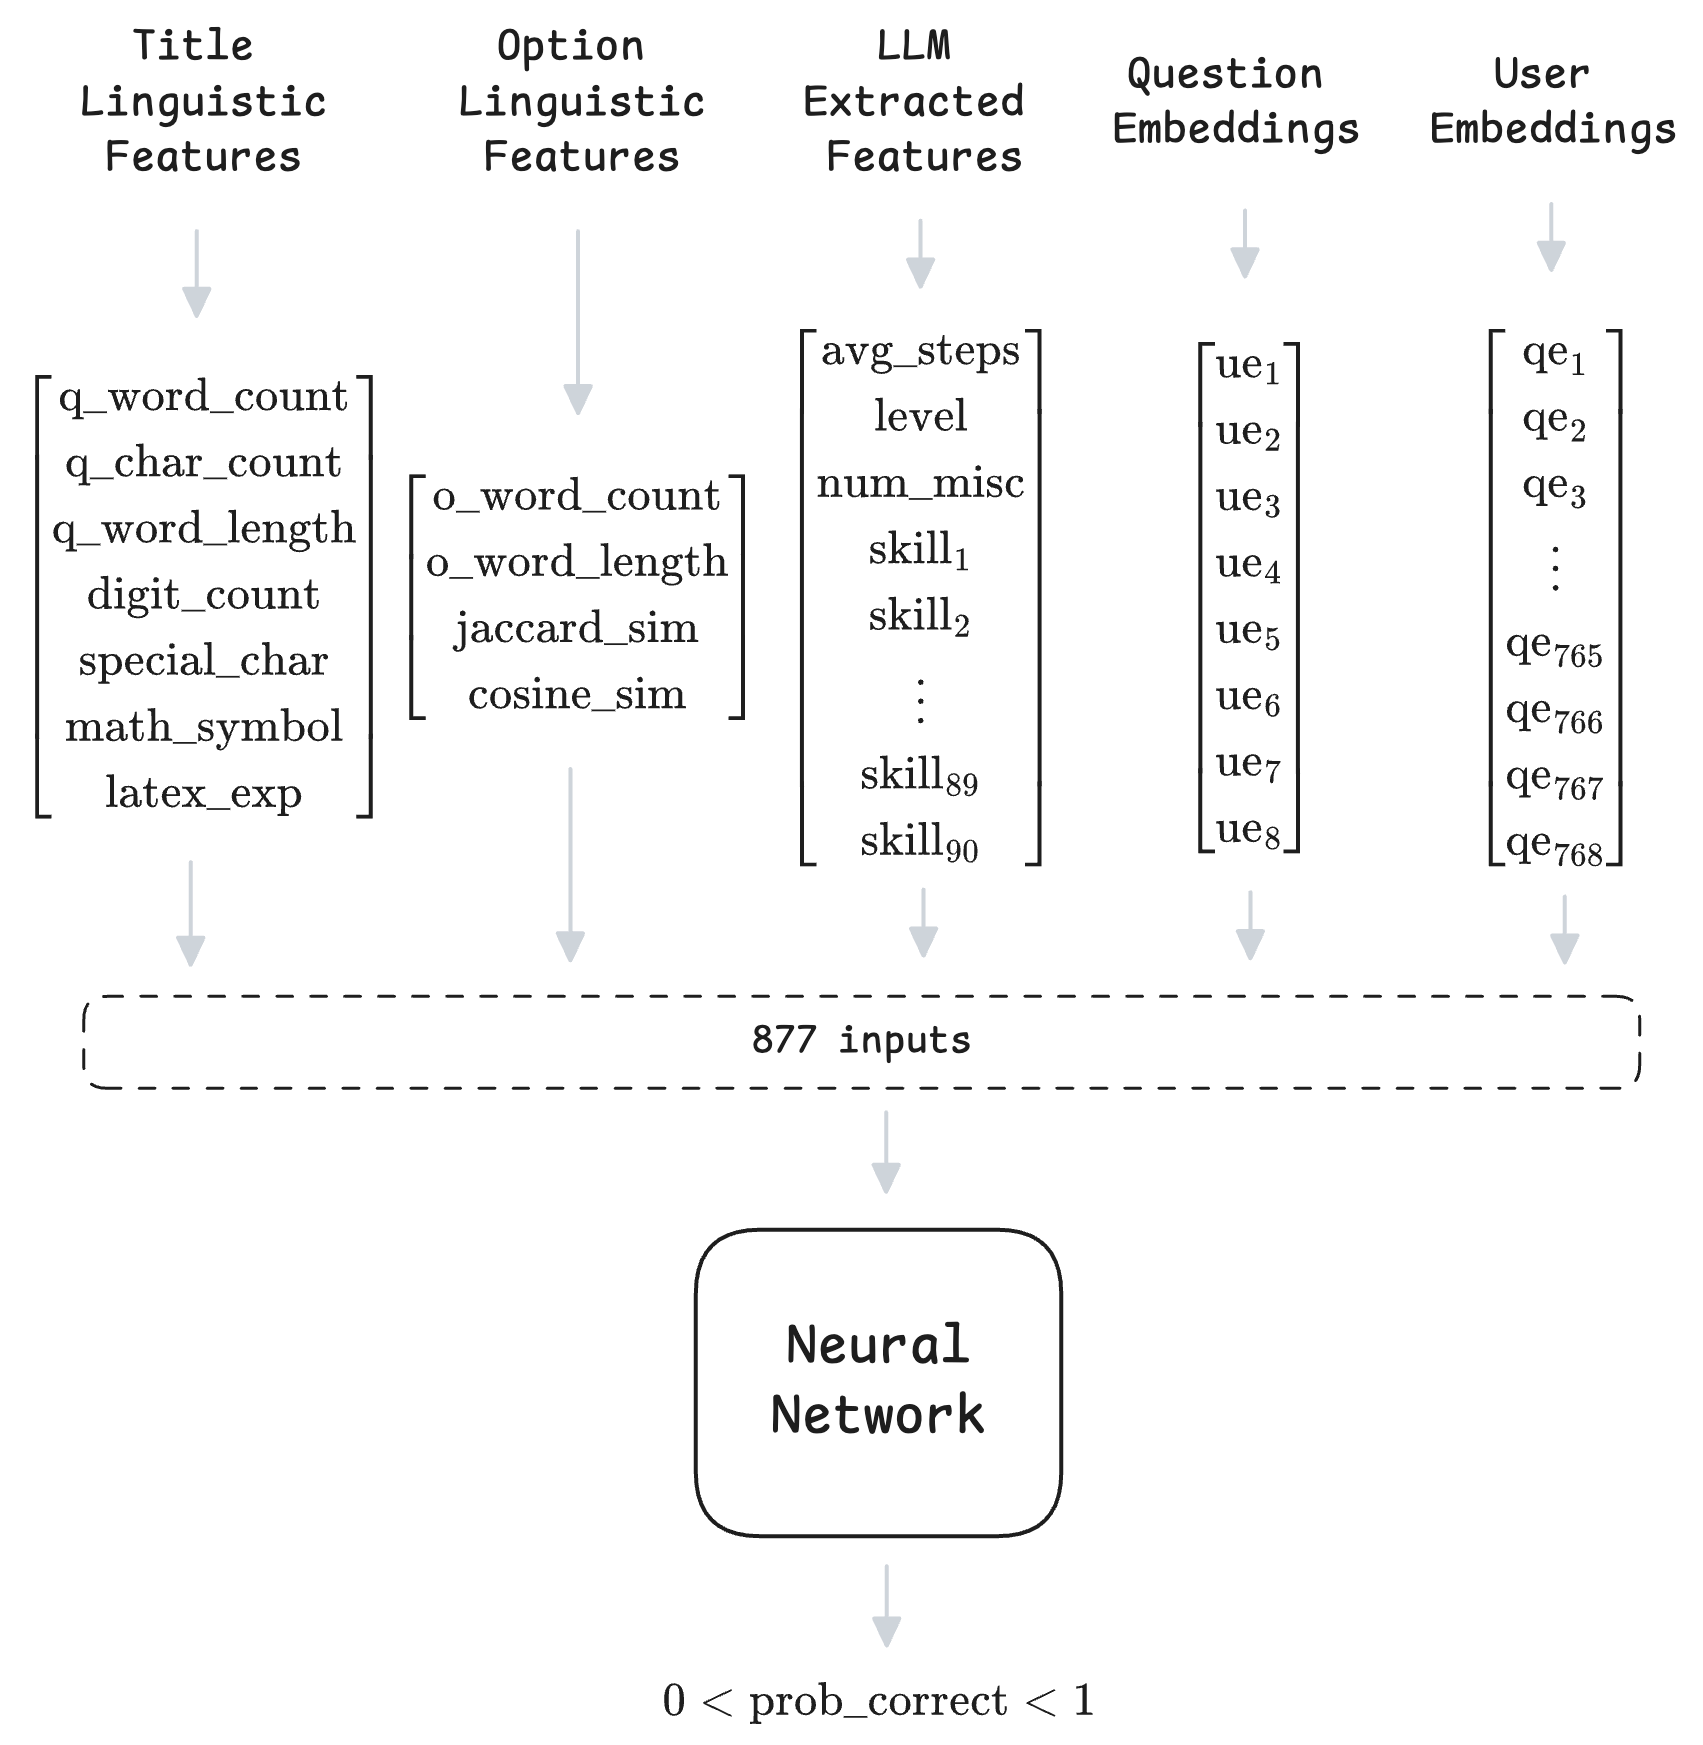
\includegraphics[width=0.8\columnwidth]{images/model_diagram.png}
    \caption{Overview of the Model Pipeline}
    \label{fig:model-pipeline}
\end{figure}

\subsection{Feature Engineering}

\subsubsection{Linguistic Features}
To capture the textual complexity and mathematical content of the questions, we extracted a set of linguistic features from the question titles and answer options.

\paragraph{Question Title Features}
We extracted the following features from the question titles:
\begin{itemize}
    \item \textbf{q\_word\_count}: Number of words in the question title. This provides a simple measure of question length, with the average question containing 23 words.
    \item \textbf{q\_char\_count}: Total number of characters in the question title. The average question contained 118 characters, with the longest having 945 characters.
    \item \textbf{q\_avg\_word\_length}: Average length of words in the title, calculated as the ratio of character count to word count. This metric helps assess the complexity of vocabulary used.
    \item \textbf{q\_digit\_count}: Number of numerical digits present in the question. This is particularly relevant for mathematics questions, which often contain numerical values.
    \item \textbf{q\_special\_char\_count}: Count of special characters in the title, excluding common punctuation. Special characters often indicate more complex notation.
    \item \textbf{q\_mathematical\_symbols}: Count of mathematical symbols (e.g., +, -, ×, ÷, =, <, >) in the question. Questions typically contained around 8 mathematical symbols on average. % Replaced \textless, \textgreater
    \item \textbf{q\_latex\_expressions}: Count of LaTeX expressions or mathematical formatting in the question, indicating the presence of complex mathematical notation.
\end{itemize}

\paragraph{Answer Option Features}
In addition to the question title, we analyzed the answer options to extract insights about their variability and length:
\begin{itemize}
    \item \textbf{jaccard\_similarity\_std}: Standard deviation of Jaccard similarities between all pairs of options. This measures how similar or different the answer options are from each other.
    \item \textbf{avg\_option\_length}: Average character length of answer options, which averaged about 10 characters.
    \item \textbf{avg\_option\_word\_count}: Average number of words in answer options, with most options containing between 1-3 words.
\end{itemize}

These linguistic features provided valuable signals for our predictive models. For example, the number of mathematical symbols and LaTeX expressions served as proxies for the mathematical complexity of questions, while features like word count and average word length helped quantify the linguistic complexity. The Jaccard similarity between answer options captured information about the discriminative power of the question, as very similar options might be more challenging for students to differentiate.

\subsubsection{Question Embeddings}

Semantic understanding of the questions is crucial for predicting student performance. To capture this, we generated embeddings of the complete question text along with its answer options using the ModernBERT model.

We formatted each question and its answer options into a structured format:
\begin{verbatim}
        Question: [question_title]
        Correct Answer: [correct_option]
        Wrong Answer 1: [wrong_option_1]
        Wrong Answer 2: [wrong_option_2]
        Wrong Answer 3: [wrong_option_3]
        Wrong Answer 4: [wrong_option_4]
    \end{verbatim} % Replaced promptbox with verbatim

The formatted text was processed through the ModernBERT model to generate 768-dimensional contextual embeddings. We applied mean pooling to combine token-level embeddings into sentence-level embeddings and normalized them to ensure consistent comparisons.


\subsubsection{Options Embeddings}

We also generated separate embeddings for each individual answer option using ModernBERT, creating 768-dimensional vectors for each of the five possible options (A through E). These embeddings captured the semantic meaning of each answer choice in isolation.

From these option embeddings, we calculated cosine similarity metrics between the correct answer and each incorrect option. For each question, we computed four similarity values (ranging from -1 to 1), creating features called \texttt{wrong\_1\_similarity} through \texttt{wrong\_4\_similarity}.

These similarity metrics provided our model with important information about the relationships between answer choices. While the question embeddings captured the overall problem context, these similarity features helped our models understand how answer options related to each other, offering insight into how specific answer choices might influence student responses.

\subsubsection{Feature Extraction Using LLMs}

In addition to traditional feature engineering and embedding techniques, we leveraged Large Language Models (LLMs) to extract pedagogically relevant features from questions that would be difficult to capture through conventional methods. We used Google's Gemini 2.0 Flash with Chain-of-Thought (CoT) prompting, requiring the model to articulate its reasoning process within \texttt{<thinking></thinking>} tags before providing the final output (see appendix). This transparency allowed us to evaluate the quality of feature extraction and ensure pedagogical validity.

\paragraph{Solution Step Count}
To quantify procedural complexity, we prompted the LLM to solve each mathematics question in the most detailed, pedagogically atomic manner possible. The LLM was instructed to break down the solution into discrete steps that would be appropriate for student instruction. For each question, we ran this extraction three separate times to account for variability. The average number of steps across these runs became a numerical feature (\texttt{avg\_steps}). This feature served as a proxy for question complexity, based on the hypothesis that questions requiring more solution steps might be more difficult.

\paragraph{Mathematical Skills}
To identify the specific mathematical knowledge required to solve each question, we created a comprehensive taxonomy of 90 common mathematical skills (see appendix). The LLM was provided with the question, answer options, and a step-by-step solution. For each question, the model identified which skills from the taxonomy were utilized in the solution. We performed this extraction five times and retained only skills that appeared in at least three runs to ensure stability. These skills were converted to one-hot encoded features, creating binary indicators for each skill.

\paragraph{Cognitive Level}
To assess the level of thinking required by each question according to Bloom's Taxonomy, we provided the LLM with a detailed rubric describing the six levels of Bloom's Taxonomy. For each question, the model determined which cognitive level (1-6, see appendix) was primarily being assessed. This process was repeated three times with majority voting to determine the final cognitive level. The resulting ordinal feature (\texttt{cognitive\_level}) captured the complexity of thinking required by each question, providing an important dimension of difficulty beyond purely mathematical complexity.

\paragraph{Misconception Count}
To understand the potential for student errors, we prompted the LLM to analyze possible misconceptions. The LLM was instructed to generate an exhaustive, atomic list of misconceptions students might have when approaching each question. This extraction was performed three times per question, and the average number of identified misconceptions became a numerical feature (\texttt{num\_misconceptions}). This feature provided insight into questions with multiple potential pitfalls, helping us quantify another dimension of question complexity.

These LLM-extracted features complemented our traditional and embedding-based features by directly capturing pedagogical aspects of the questions. By using multiple runs and aggregation techniques (averaging or majority voting), we ensured the stability and reliability of these features.

\subsubsection{User Embeddings}

The last piece of the puzzle in our modeling approach was incorporating user information, since we had student answer data for each question. Accounting for individual student abilities was essential for accurate predictions.

We implemented a neural network with a dedicated user embedding layer that mapped each user ID to an 8-dimensional vector space. This approach reduced the feature dimensionality while creating dense, continuous representations of user abilities. The embedding layer contained a learnable matrix of dimensions $(n\_users \times embedding\_dim)$ that captured latent ability factors conventional one-hot encoding could not efficiently represent. This embedding-based approach successfully balanced user and question influences, enabling our model to make meaningfully different predictions for different questions presented to the same user, while ensuring user characteristics did not overshadow the question features we were primarily interested in analyzing.

\subsection{Modeling Approach}

We developed a neural network architecture specifically designed to balance the influence of user characteristics and question features.

Our model combines user embeddings (dimensions: $n\_users \times 8$), question numerical features, and question embeddings into a single concatenated feature vector. This combined representation is then passed through two dense layers with 64 and 32 units respectively, applying dropout rates of 0.3 and 0.2 to prevent overfitting. The network concludes with a sigmoid output layer that predicts the probability of a correct answer, effectively balancing the contributions of both user abilities and question characteristics.

For modeling purposes, we implemented a robust three-way split at the question level rather than row level:

\begin{itemize}
    \item \textbf{Training set}: 3,275 questions (70\%) used for model training
    \item \textbf{Validation set}: 937 questions (20\%) used for model tuning and performance assessment
    \item \textbf{Holdout test set}: 469 questions (10\%) saved for final evaluation
\end{itemize}

\subsection{Prediction Task}

While our neural network achieved strong classification performance, our primary research objective extended beyond merely predicting student responses. The ultimate goal was to use these predictions to estimate question difficulty parameters in a way that aligns with Item Response Theory (IRT), a foundational framework in educational assessment.

After training the neural network on 70\% of the questions and validating on 20\%, we used the model to generate predictions for the 10\% completely unseen questions in the holdout test set. For each of the 469 holdout questions, we generated predictions for all 1,867 users. We first preserved the raw probability outputs from the model, representing each student's likelihood of answering correctly. We then applied a 0.5 threshold to these probabilities to convert them to binary predictions (0 for incorrect, 1 for correct). This conversion produced a correctness matrix where each cell contained either 0 or 1, representing whether a specific user would answer a specific question correctly.

We then used these correctness matrices as inputs to an Item Response Theory estimation process. We implemented a 2-Parameter Logistic (2PL) IRT model using PyTorch to estimate three key parameters: question difficulty (how challenging each question is), question discrimination (how well each question differentiates between ability levels), and user ability (the proficiency level of each user). These parameters are related through the IRT equation $P(\text{correct}) = \sigma(a(\theta - b))$, where $\sigma$ is the logistic function. The parameter estimation employed a maximum likelihood approach, where parameters were initialized as random values with small variance and optimized using the Adam optimizer with a learning rate of 0.01 and weight decay of $1e-5$. We used a learning rate scheduler that reduced the rate by half when progress plateaued, and the optimization process ran for up to 5,000 iterations with early stopping.

After estimating the parameters, we compared them to the ground truth difficulty parameters from the original dataset.

\section{Results}

\subsection{Model Performance}

Our neural network model achieved strong performance on the prediction task, effectively balancing the influence of user characteristics and question features. Classification metrics on the validation set demonstrated the model's ability to accurately predict student responses to unseen questions.

\begin{table}[!ht] % Changed from [H]
  \centering
  \begin{tabular}{lc}
        \toprule % Use booktabs
        \textbf{Metric} & \textbf{Value} \\
        \midrule % Use booktabs
        Accuracy & 78.15\% \\
        Precision & 82.18\% \\
        Recall & 88.12\% \\
        F1 Score & 85.04\% \\
        AUC-ROC & 0.8197 \\
        \bottomrule % Use booktabs
  \end{tabular}
    \caption{Classification performance metrics on the validation set.}
    \label{tab:classification-metrics}
\end{table}

The classification metrics indicate that our model performs well at predicting individual student responses, with an accuracy of 78.15\% on the validation set. The higher precision (82.18\%) compared to accuracy suggests that when the model predicts a student will answer correctly, it is usually right. The recall of 88.12\% indicates the model successfully identifies most instances where students would answer correctly. The F1 score of 85.04\% represents a strong balance between precision and recall. The AUC-ROC value of 0.8197 further confirms the model's ability to distinguish between correct and incorrect responses across different threshold settings.

These results are particularly encouraging as they confirm that our model is effectively leveraging both question features and student characteristics. The strong classification performance indicates the model is capturing sufficient signal from student features to modify its predictions based on individual student abilities, while simultaneously accounting for inherent question characteristics. This balanced approach provides a solid foundation for the subsequent IRT parameter estimation, as accurate response predictions that account for both question difficulty and student proficiency are essential for deriving reliable difficulty parameters.

\subsection{IRT Parameter Estimation}

Beyond direct prediction performance, our primary research objective was to accurately estimate Item Response Theory (IRT) difficulty parameters for unseen questions. Our neural network approach demonstrated exceptional performance on this task.

When applying our model to the completely unseen questions in the holdout test set using predictions from all 1,867 users, we achieved alignment between estimated and true difficulty parameters:

\begin{table}[!ht] % Changed from [H]
    \centering
  \begin{tabular}{lc}
        \toprule % Use booktabs
        \textbf{Metric} & \textbf{Value} \\
        \midrule % Use booktabs
        Pearson correlation & 0.8549 \\
        Spearman rank correlation & 0.9629 \\
        Mean Absolute Error (MAE) & 0.6286 \\
        Root Mean Square Error (RMSE) & 1.0760 \\
        \bottomrule % Use booktabs
  \end{tabular}
    \caption{IRT parameter estimation metrics on the holdout test set.}
    \label{tab:irt-metrics}
\end{table}

The high correlation values (Pearson > 0.85, Spearman > 0.96) demonstrate that the difficulty estimations derived from our predicted student responses strongly align with the ground truth parameters.

\begin{figure}[!ht] % Changed from [H]
    \centering
    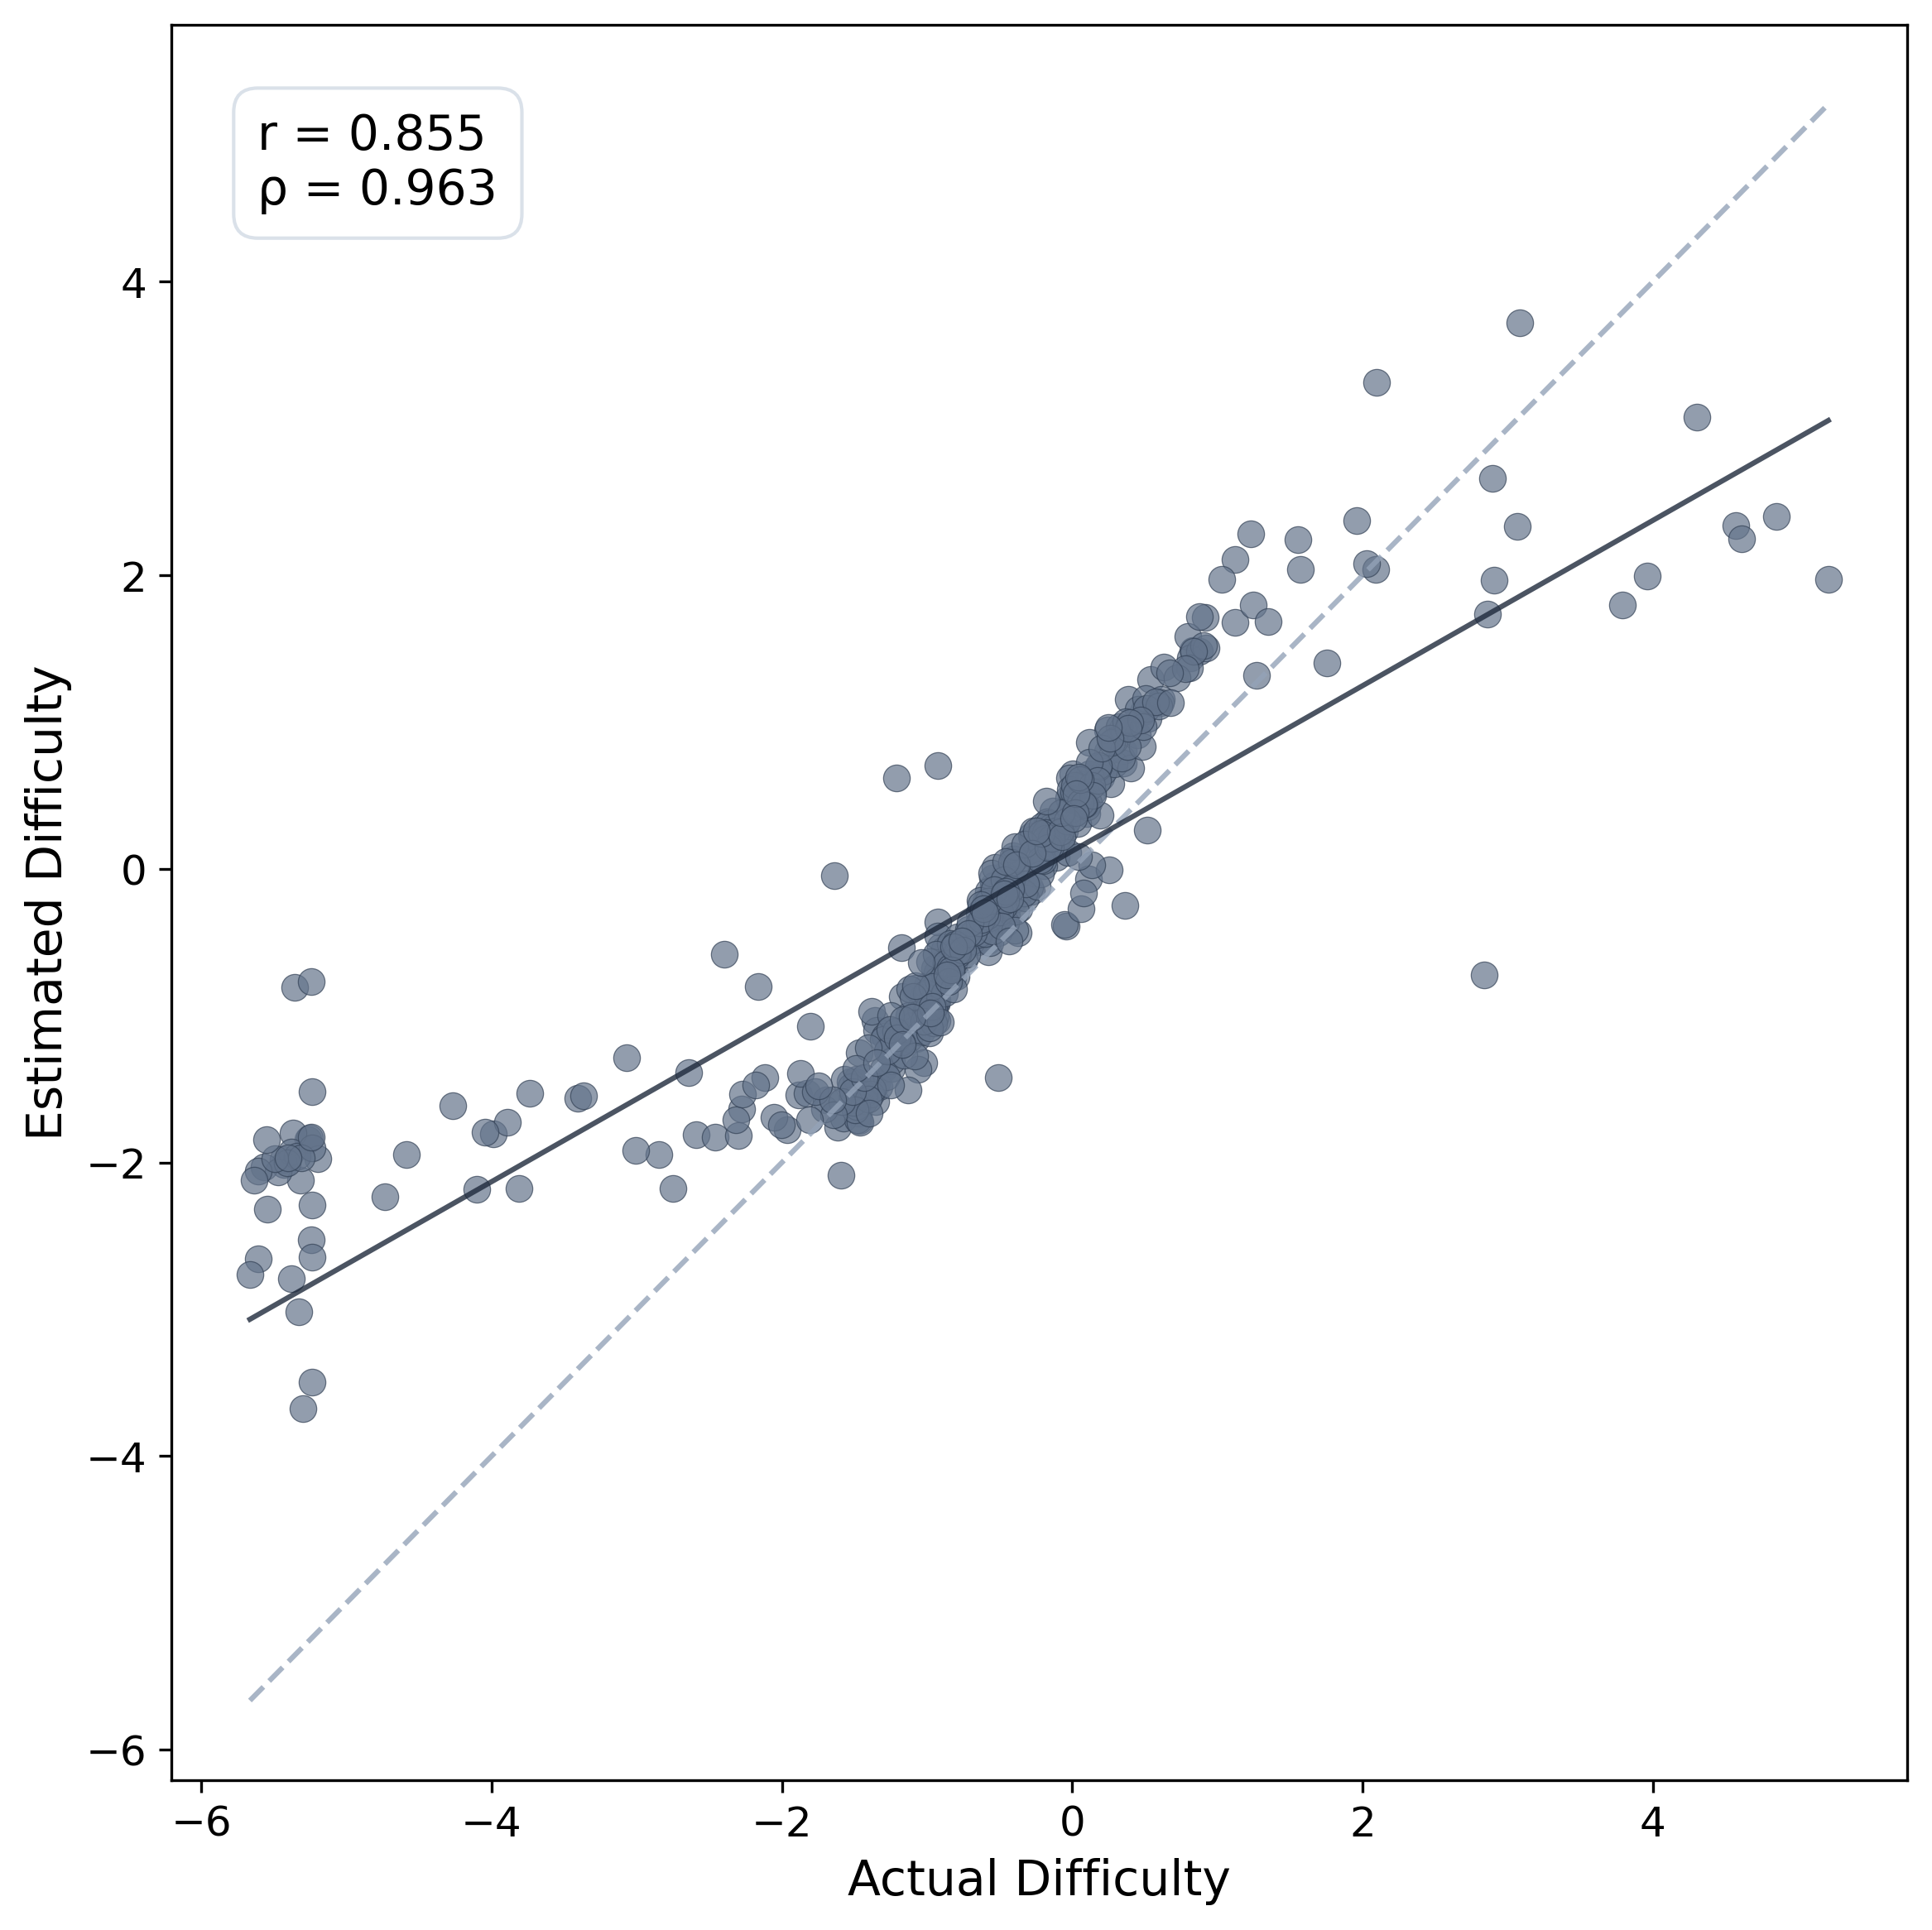
\includegraphics[width=1\columnwidth]{../../one_model_experiment/figures/difficulty_comparison.png}
    \caption{Correlation between original and estimated IRT difficulty parameters showing strong linear relationship across the entire difficulty spectrum.}
    \label{fig:difficulty-correlation}
\end{figure}

As shown in Figures~\ref{fig:difficulty-correlation} and~\ref{fig:difficulty-distribution}, our model captures both the relative ordering and the absolute scaling of question difficulties. The strong linear relationship in Figure~\ref{fig:difficulty-correlation} confirms the high correlation metrics, while Figure~\ref{fig:difficulty-distribution} demonstrates that the distributions of estimated and true difficulty parameters align remarkably well, preserving the overall shape and range found in the original dataset.

\begin{figure}[!ht] % Changed from [H]
  \centering
    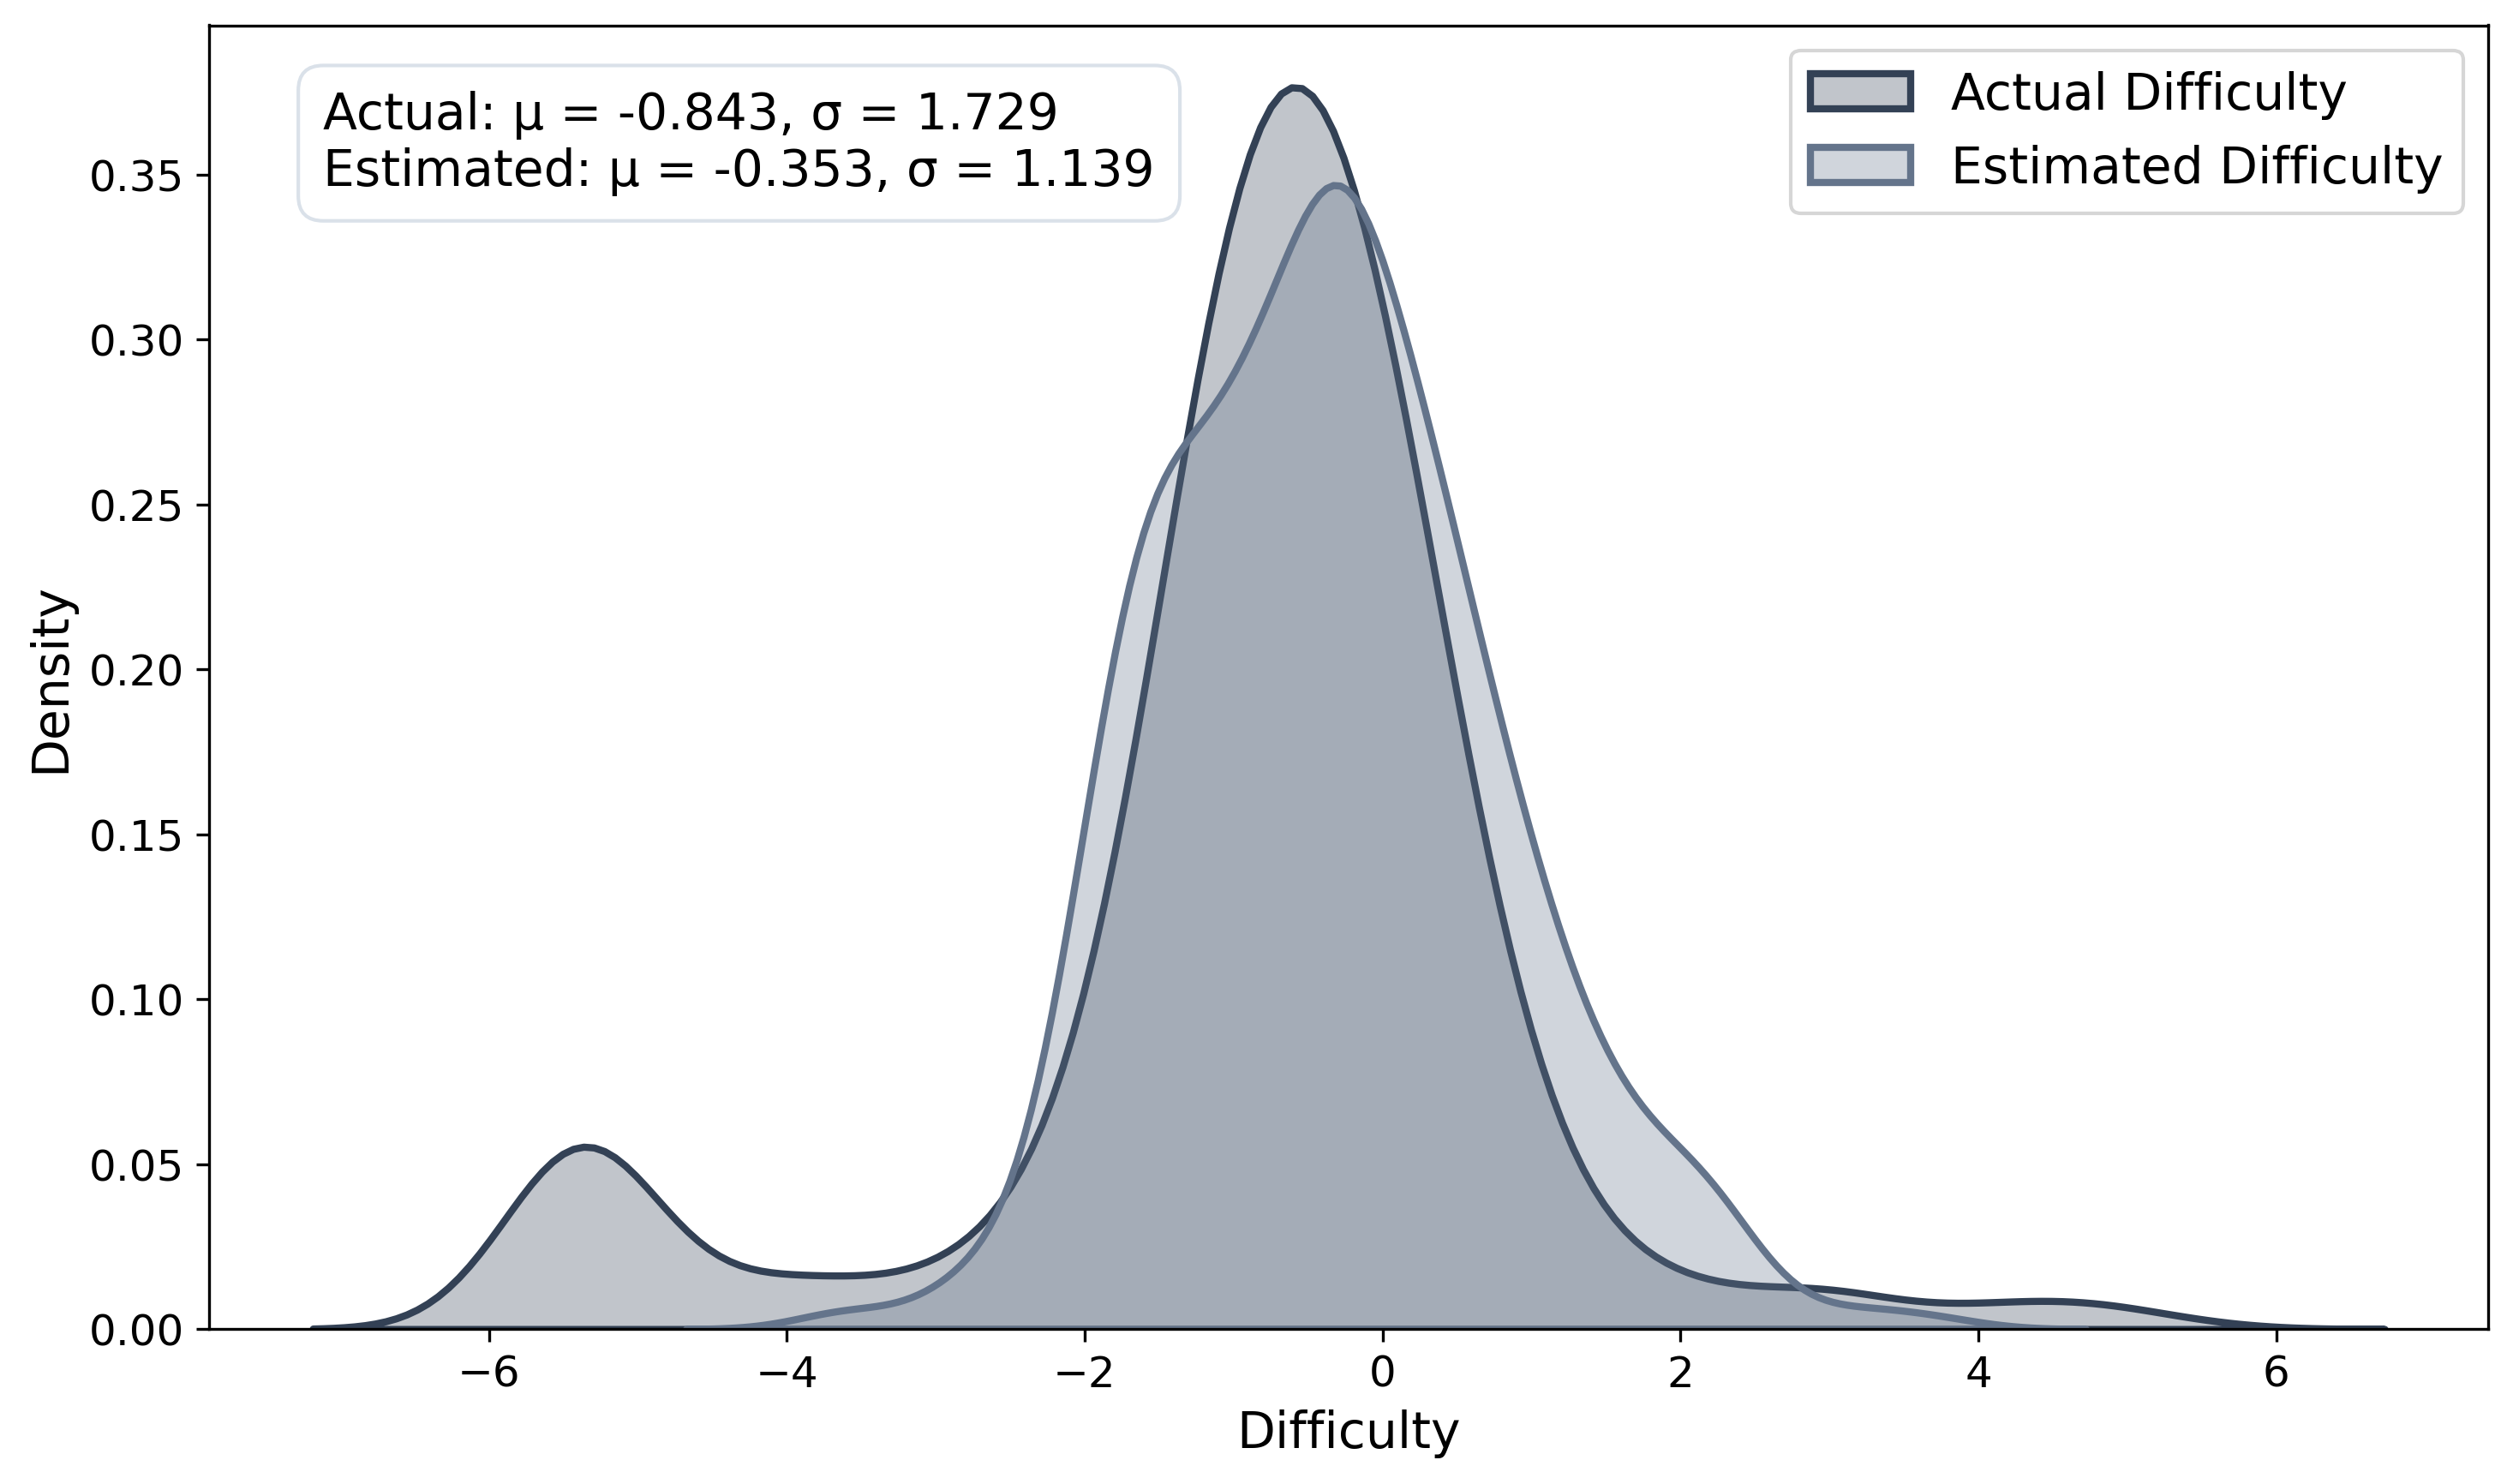
\includegraphics[width=1\columnwidth]{../../one_model_experiment/figures/difficulty_distributions.png}
    \caption{Distribution comparison of original and estimated difficulty parameters demonstrating close alignment in both shape and range.}
    \label{fig:difficulty-distribution}
\end{figure}

This evaluation demonstrates that our neural network approach achieved its primary objective: accurately estimating question difficulty parameters for completely unseen questions, by predicting student responses to those questions.

\section{Discussion}

\subsection{Conclusions}

Our research demonstrates that Item Response Theory difficulty parameters can be accurately estimated without traditional student testing by combining linguistic features with pedagogical insights extracted using Large Language Models. This approach addresses a significant challenge in educational assessment: the need for efficient methods to determine question difficulty that don't rely on resource-intensive pre-testing with students.

The strong performance of our neural network model in predicting student responses (78.15\% accuracy, 85.04\% F1 score) confirms that our feature engineering approach effectively captures the factors that influence student performance on mathematics questions. By integrating traditional linguistic features, semantic embeddings, and LLM-extracted pedagogical insights, we created a representation of question characteristics that allowed our model to make accurate predictions.

Most importantly, when presented with completely unseen questions, our model generated response patterns so reliable that we could predict question difficulties with remarkable accuracy (Pearson correlation of 0.85). These high correlations demonstrate that our approach can effectively capture both the relative ordering and absolute scaling of question difficulties without requiring actual student testing.

\section*{Limitations}

Despite the promising results, several limitations of our study should be acknowledged:

\paragraph{Generalizability}: Our dataset originates from Chile, which may limit the generalizability of our findings to student populations elsewhere. Educational systems, curricula, and pedagogical approaches vary across countries and cultures, potentially affecting how question features relate to difficulty in different contexts.

\paragraph{LLM Stability}: Large Language Models are inherently probabilistic. Even though we attempted to ensure stability by making multiple LLM calls and aggregating results, each new call could potentially yield different outputs. This variability introduces some uncertainty into the LLM-extracted features, which could affect the consistency of our predictions.

\paragraph{Model Interpretability}: The neural network we employed is essentially a black box that performs well on the prediction task but offers limited insight into the relative importance of different features. This lack of interpretability makes it difficult to draw definitive conclusions about which specific question characteristics contribute most significantly to difficulty.

\paragraph{Model Sensitivity}: Additionally, our results may vary depending on which LLM vendor we use (e.g., OpenAI, Anthropic, Google) and which inference parameters we select (e.g., temperature, top-p sampling). These choices can significantly impact the quality and consistency of the LLM-extracted features that feed into our model.

\paragraph{Skill Taxonomy}: The mathematical skill taxonomy we used was created specifically for this study rather than drawing on a standardized, widely accepted framework. This limits comparability with other research and raises questions about the comprehensiveness and validity of our skill categorization.

\bibliography{custom}

\appendix

\section{Appendix}

\subsection{Step by Step Example}
\label{sec:step-by-step-example}
The following is an example prompt used to generate step by step solution explanations for a mathematical problem:

\begin{quote} % Replaced questionbox
    \textbf{Prompt} \\
    You are an expert in math pedagogy. Your task is to answer the following question deconstructing it to the most elemental steps. Don't skip any step. Don't assume anything about the reader, try to solve it in the most atomic and pedagogical way possible.

    \vspace{1em}

    Here is the question:
    \vspace{1em}

    Question: What is the decreasing order of the roots $4\sqrt{3}$, $3\sqrt{4}$, $2\sqrt{5}$, and $5\sqrt{2}$?

    A) $2\sqrt5 > 4\sqrt3 > 5\sqrt2 > 3\sqrt4$

    B) $2\sqrt5 > 3\sqrt4 > 4\sqrt3 > 5\sqrt2$

    C) $5\sqrt2 > 3\sqrt4 > 4\sqrt3 > 2\sqrt5$

    D) $5\sqrt2 > 4\sqrt3 > 3\sqrt4 > 2\sqrt5$

    E) $2\sqrt5 > 4\sqrt3 > 5\sqrt2 > 3\sqrt4$

    Correct Answer: D

    \vspace{1em}

    First, think about your task step by step inside <thinking></thinking> tags. Your thinking process should try to go over all the posible ways to solve the question and try to find the most atomic way to solve it.

    \vspace{1em}

    Then, when you are ready to answer, after your </thinking> tag you should write your response using "Step" as the key and the step as the value. For example:

    \vspace{1em}

    <thinking>

      Thinking process... Think as long as you need to.

    </thinking>

    \vspace{1em}

    Step 1: ...

    Step 2: ...

    Step 3: ...

    ...

    \vspace{1em}

    Important instructions:

    - Don't skip any step.

    - Don't assume anything about the reader, try to solve it in the most atomic and pedagogical way possible.

    - Use as many steps as you need to.
\end{quote}

And here is the LLM's response:

\begin{quote} % Replaced studentbox
    \textbf{Thinking Process} \\
    <thinking>

    Okay, let's break down this problem. We need to compare four numbers:  $4\sqrt3$, $3\sqrt4$, $2\sqrt5$, and $5\sqrt2$ and arrange them in decreasing order. The main challenge is that the numbers are in a mixed form (integer multiplied by a square root). To compare them easily, we need to get rid of the square roots or the integers outside the square root.

    \vspace{1em}

    The easiest way to compare these values is to bring the coefficients *inside* the square root.

    \vspace{1em}

    Let's consider how to bring a number inside a square root. For example, consider $a\sqrt{b}$. We can rewrite this as $\sqrt{a^2 * b}$.

    \vspace{1em}

    So, the first step is to convert all the numbers into the form of a single square root.

    \vspace{1em}

    Then, we simply compare the numbers *inside* the square roots, because if $a > b$, then $\sqrt{a} > \sqrt{b}$.

    \vspace{1em}

    Finally, we arrange the original numbers based on their corresponding squared values, in decreasing order.

    \vspace{1em}

    Let's start the solution.

    </thinking>

    \vspace{1em}
\end{quote}

\begin{quote} % Replaced llmbox
    \textbf{Response} \\
    Step 1: Convert $4\sqrt3$ into the form $\sqrt{x}$.

    We have $4\sqrt3 = \sqrt{4^2 * 3} = \sqrt{16 * 3} = \sqrt{48}$

    \vspace{1em}

    Step 2: Convert $3\sqrt4$ into the form $\sqrt{x}$.

    We have $3\sqrt4 = \sqrt{3^2 * 4} = \sqrt{9 * 4} = \sqrt{36}$

    \vspace{1em}

    Step 3: Convert $2\sqrt5$ into the form $\sqrt{x}$.

    We have $2\sqrt5 = \sqrt{2^2 * 5} = \sqrt{4 * 5} = \sqrt{20}$

    \vspace{1em}

    Step 4: Convert $5\sqrt2$ into the form $\sqrt{x}$.

    We have $5\sqrt2 = \sqrt{5^2 * 2} = \sqrt{25 * 2} = \sqrt{50}$

    \vspace{1em}

    Step 5: Now we have $\sqrt{48}$, $\sqrt{36}$, $\sqrt{20}$, and $\sqrt{50}$. We can easily compare the values inside the square roots: 48, 36, 20, and 50.

    \vspace{1em}

    Step 6: Arrange the values inside the square roots in decreasing order:

    50 > 48 > 36 > 20

    \vspace{1em}

    Step 7: Replace the values inside the square roots with their original forms:

    $5\sqrt2 > 4\sqrt3 > 3\sqrt4 > 2\sqrt5$

    \vspace{1em}

    Step 8: Compare this result with the given options.

    The correct option is D: $5\sqrt2 > 4\sqrt3 > 3\sqrt4 > 2\sqrt5$.
\end{quote}

\subsection{Mathematical Skill List}
\label{tab:math-skills} % Keep label for potential cross-referencing
The following table presents the list of mathematical skills assessed in our dataset for our skill one-hot encoding.

\vspace{1em}

% Using longtable for the skills list as it's long
\begin{table}
\centering
\caption{Mathematical skills assessed in the dataset (Part 1).}
\begin{tabular}{p{0.45\columnwidth}p{0.45\columnwidth}}
\toprule
\textbf{Skill} & \textbf{Category} \\
\midrule

% First part of the table - we'll split it into multiple tables
Addition & Arithmetic/Number Sense \\
Subtraction & Arithmetic/Number Sense \\
Multiplication & Arithmetic/Number Sense \\
Division & Arithmetic/Number Sense \\
Mental Math & Arithmetic/Number Sense \\
Estimation & Arithmetic/Number Sense \\
Number Properties & Arithmetic/Number Sense \\
Fractions & Arithmetic/Number Sense \\
Decimals & Arithmetic/Number Sense \\
Percentages & Arithmetic/Number Sense \\
Factors and Multiples & Arithmetic/Number Sense \\
Order of Operations & Arithmetic/Number Sense \\
\bottomrule
\end{tabular}
\end{table}

\begin{table}
\centering
\caption{Mathematical skills assessed in the dataset (Part 2).}
\begin{tabular}{p{0.45\columnwidth}p{0.45\columnwidth}}
\toprule
\textbf{Skill} & \textbf{Category} \\
\midrule
Ratios & Ratios Proportions Rates \\
Proportions & Ratios Proportions Rates \\
Rates & Ratios Proportions Rates \\
Unit Conversions & Ratios Proportions Rates \\
Scale Factors & Ratios Proportions Rates \\
Variables and Expressions & Algebra \\
Linear Equations & Algebra \\
Systems of Equations & Algebra \\
Inequalities & Algebra \\
Polynomials & Algebra \\
Factoring & Algebra \\
Quadratic Equations & Algebra \\
\bottomrule
\end{tabular}
\end{table}

\begin{table}
\centering
\caption{Mathematical skills assessed in the dataset (Part 3).}
\begin{tabular}{p{0.45\columnwidth}p{0.45\columnwidth}}
\toprule
\textbf{Skill} & \textbf{Category} \\
\midrule
Exponents and Radicals & Algebra \\
Rational Expressions & Algebra \\
Logarithms & Algebra \\
Function Notation & Functions and Graphing \\
Domain and Range & Functions and Graphing \\
Linear Functions & Functions and Graphing \\
Quadratic Functions & Functions and Graphing \\
Polynomial Functions & Functions and Graphing \\
Exponential Functions & Functions and Graphing \\
Logarithmic Functions & Functions and Graphing \\
Piecewise Functions & Functions and Graphing \\
Function Transformations & Functions and Graphing \\
\bottomrule
\end{tabular}
\end{table}

\begin{table}
\centering
\caption{Mathematical skills assessed in the dataset (Part 4).}
\begin{tabular}{p{0.45\columnwidth}p{0.45\columnwidth}}
\toprule
\textbf{Skill} & \textbf{Category} \\
\midrule
Function Composition & Functions and Graphing \\
Angles & Geometry \\
Triangles & Geometry \\
Quadrilaterals & Geometry \\
Polygons & Geometry \\
Circles & Geometry \\
Area and Perimeter & Geometry \\
Volume and Surface Area & Geometry \\
Coordinate Geometry & Geometry \\
Transformations & Geometry \\
Pythagorean Theorem & Geometry \\
Similar Triangles & Geometry \\
\bottomrule
\end{tabular}
\end{table}

\begin{table}
\centering
\caption{Mathematical skills assessed in the dataset (Part 5).}
\begin{tabular}{p{0.45\columnwidth}p{0.45\columnwidth}}
\toprule
\textbf{Skill} & \textbf{Category} \\
\midrule
Congruence & Geometry \\
Geometric Constructions & Geometry \\
Geometric Proofs & Geometry \\
Basic Trigonometric Ratios & Trigonometry \\
Inverse Trigonometric Functions & Trigonometry \\
Unit Circle & Trigonometry \\
Trigonometric Identities & Trigonometry \\
Law of Sines/Cosines & Trigonometry \\
Polar Coordinates & Trigonometry \\
Mean Median Mode & Statistics and Probability \\
Range and Standard Deviation & Statistics and Probability \\
Data Representation & Statistics and Probability \\
\bottomrule
\end{tabular}
\end{table}

\begin{table}
\centering
\caption{Mathematical skills assessed in the dataset (Part 6).}
\begin{tabular}{p{0.45\columnwidth}p{0.45\columnwidth}}
\toprule
\textbf{Skill} & \textbf{Category} \\
\midrule
Basic Probability & Statistics and Probability \\
Compound Probability & Statistics and Probability \\
Conditional Probability & Statistics and Probability \\
Combinatorics & Statistics and Probability \\
Statistical Inference & Statistics and Probability \\
Regression Analysis & Statistics and Probability \\
Hypothesis Testing & Statistics and Probability \\
Limits & Calculus \\
Derivatives & Calculus \\
Integrals & Calculus \\
Applications of Calculus & Calculus \\
Word Problem Translation & Problem Solving \\
\bottomrule
\end{tabular}
\end{table}

\begin{table}
\centering
\caption{Mathematical skills assessed in the dataset (Part 7).}
\begin{tabular}{p{0.45\columnwidth}p{0.45\columnwidth}}
\toprule
\textbf{Skill} & \textbf{Category} \\
\midrule
Multi-step Problem Solving & Problem Solving \\
Mathematical Modeling & Problem Solving \\
Logical Reasoning & Problem Solving \\
Pattern Recognition & Problem Solving \\
Complex Numbers & Advanced Topics \\
Matrices & Advanced Topics \\
Sequences and Series & Advanced Topics \\
Vector Geometry & Advanced Topics \\
Set Theory & Discrete Mathematics \\
Graph Theory & Discrete Mathematics \\
Financial Mathematics & Applied Mathematics \\
Technology in Mathematics & Tools and Technology \\
Mathematical Communication & Meta Skills \\
Mathematical Literacy & Meta Skills \\
\bottomrule
\end{tabular}
\end{table}

\subsection{Bloom's Cognitive Level Table}
Table \ref{tab:blooms-taxonomy} outlines Bloom's Taxonomy levels used to classify the cognitive demands of problems. Each level is an ordinal number in our feature encoding.
\begin{table}[!ht] % Changed from [H]
    \centering
    \begin{tabular}{p{0.30\columnwidth}p{0.60\columnwidth}} % Adjusted width slightly
        \toprule % Use booktabs
        \textbf{Cognitive Level} & \textbf{Description} \\
        \midrule % Use booktabs
        Remember & Recall facts and basic concepts \\
        Understand & Explain ideas or concepts, interpret, summarize \\
        Apply & Use information in new situations, execute procedures \\
        Analyze & Draw connections among ideas, break down into parts \\
        Evaluate & Justify a stand or decision, verify, critique \\
        Create & Produce new or original work, design, construct \\
        \bottomrule % Use booktabs
    \end{tabular}
    \caption{Bloom's Taxonomy of cognitive levels applied to mathematical problem classification.}
    \label{tab:blooms-taxonomy}
\end{table}

\subsection{Example of Misconceptions List}
Following the example from the appendix \ref{sec:step-by-step-example}, here is one of the outputs of the LLM when asked about common misconceptions for the question in the example.

\begin{enumerate} % Standard enumerate
    \item Students may confuse 'decreasing order' with 'increasing order', leading them to reverse the correct order of the numbers.
    \item Students might incorrectly apply the property $a\sqrt{b} = \sqrt{a^2 * b}$ by forgetting to square 'a' before multiplying by 'b', calculating it as $a\sqrt{b} = \sqrt{a * b}$.
    \item Students might make arithmetic errors when squaring the number outside the square root (e.g., calculating $4^2$ as 8 instead of 16).
    \item Students might make arithmetic errors in the multiplication step within the square root (e.g., calculating $16 * 3$ as 45 instead of 48).
    \item Students may believe that the magnitude of the number outside the square root is the primary determinant of the overall value, even if the value inside the square root is smaller (e.g., incorrectly assuming that $5\sqrt{2}$ is always greater than $2\sqrt{5}$ because 5 > 2).
    \item After correctly comparing the values under the square roots, students might forget to convert them back to their original forms when selecting the final answer, leading them to choose an option with the numbers under the square roots ordered.
    \item Students might make careless copying errors when transferring the correctly ordered expressions from their intermediate steps to the final answer choice.
    \item Students may lack a strong number sense regarding the approximate values of square roots, making it difficult to estimate and compare the values without performing the conversion to a common form.
    \item Students may struggle with the concept that irrational numbers can be ordered on a number line, treating them as inherently harder to compare than integers.
    \item Students might try to apply the square root individually to each term, incorrectly stating that $a\sqrt{b} = \sqrt{a} * \sqrt{b}$.
    \item Students might not understand what a root is and how it affects the order of the numbers.
\end{enumerate}

This was performed 3 times and then averaged the number of misconceptions for each question.

\end{document}
